\documentclass[12pt] {article}
\usepackage[top=1.75in, bottom=1.75in, left=1.75in, right=1.75in]{geometry}
\usepackage[pdftex]{hyperref}
\usepackage{graphicx}
\usepackage{placeins}

\hypersetup{
	pdfauthor={Phil Monroe and Kramer Straube},
	pdftitle={EEC 277 Project 2}}
	
\begin{document}

\title{EEC 277 Project 2}
\author{Phil Monroe and Kramer Straube}
\date{Feb. 6, 2012}
\maketitle

% Intro -----------------------------------------------------------------------
\section {Introduction}
In this report, we will describe the series of tests we performed to characterize various aspects of the graphics card, namely the EVGA NVIDIA 9500 GT. Some basic statistics about this card are that the GPU contains 4 multiprocessors with 8 cores each. Since this GPU supports NVIDIA CUDA compute capability version 1.1, it can support up to 768 threads per multiprocessor. In section 2, we will cover how the graphical load of the GPU is affected by different variables. In section 3, we will examine the statistics of the compute capabilities of this particular graphics card.

% Part A ----------------------------------------------------------------------
\newpage
\section{Part A}
In this section, we will discuss the way different input data sets and settings can affect the graphical capabilities of the graphics card using OpenGL and the instructional version of WesBench.
\subsection{Triangle Area}
This test iterates through various triangle areas to determine how the fill rate and vertex rate change. The data, as shown in Figure 1, shows how this graphics card handles the change in triangle area size. The fill rate flattens out as it gets larger, which is a sign that the rasterizer is getting maxed out. The vertex rate stays steady in the beginning since primitive assembly is maxed out. It then declines as the area increases because there are fewer vertices overall. The crossover where the rasterizer becomes the bottleneck over primitive assembly is at 64px.
\begin{figure}[ht!]
	\centering
	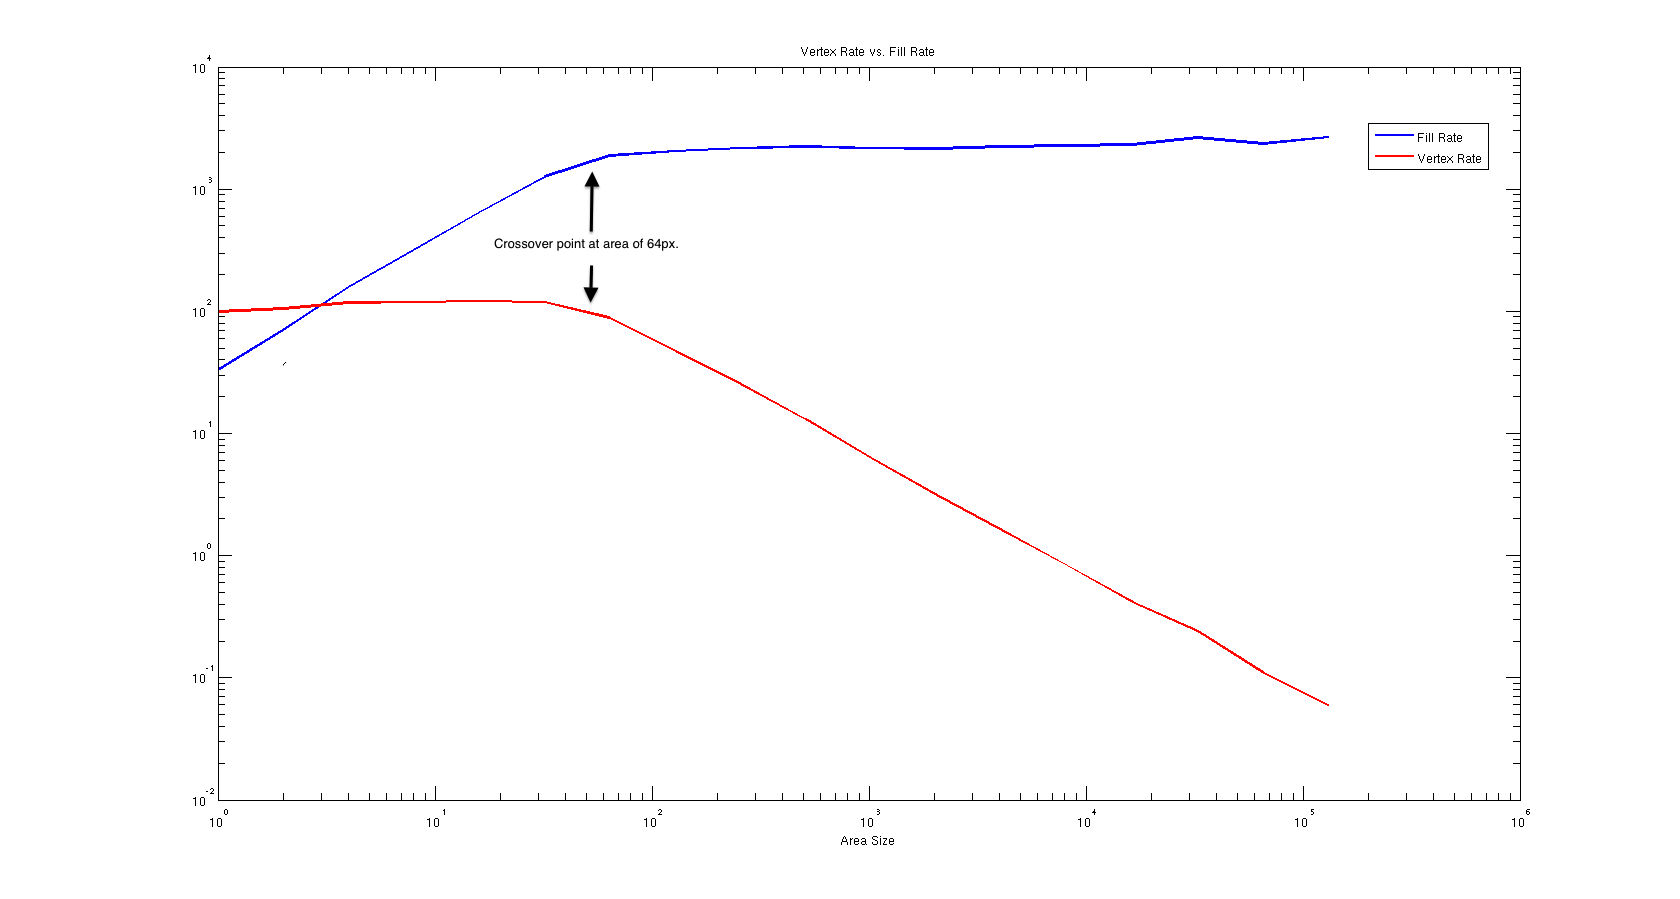
\includegraphics[width=5in]{figures/results1.png}
	\caption{Vertex rate and fill rate for various triangle areas.}
\end{figure}
\FloatBarrier

\newpage
\subsection{Lighting and Texture}
This test shows the effects of enabling lighting and texturing the triangles. Figure 2 shows that the lighting has relatively little effect on the graphics performance of this card. This is likely due to the specialized lighting hardware on the GPU. Texturing, as shown in Figure 3, drops the graphics performance a bit, but still has a minor impact. Figure 4 shows the effects of enabling both texture and lighting, which is similar to the texture test. This is due to the fact that the effect of lighting is negligible to the effect of texturing. Therefore, adding texture and lighting have no effect on the rasterization vs. primitive assembly crossover point.
\begin{figure}[ht!]
	\centering
	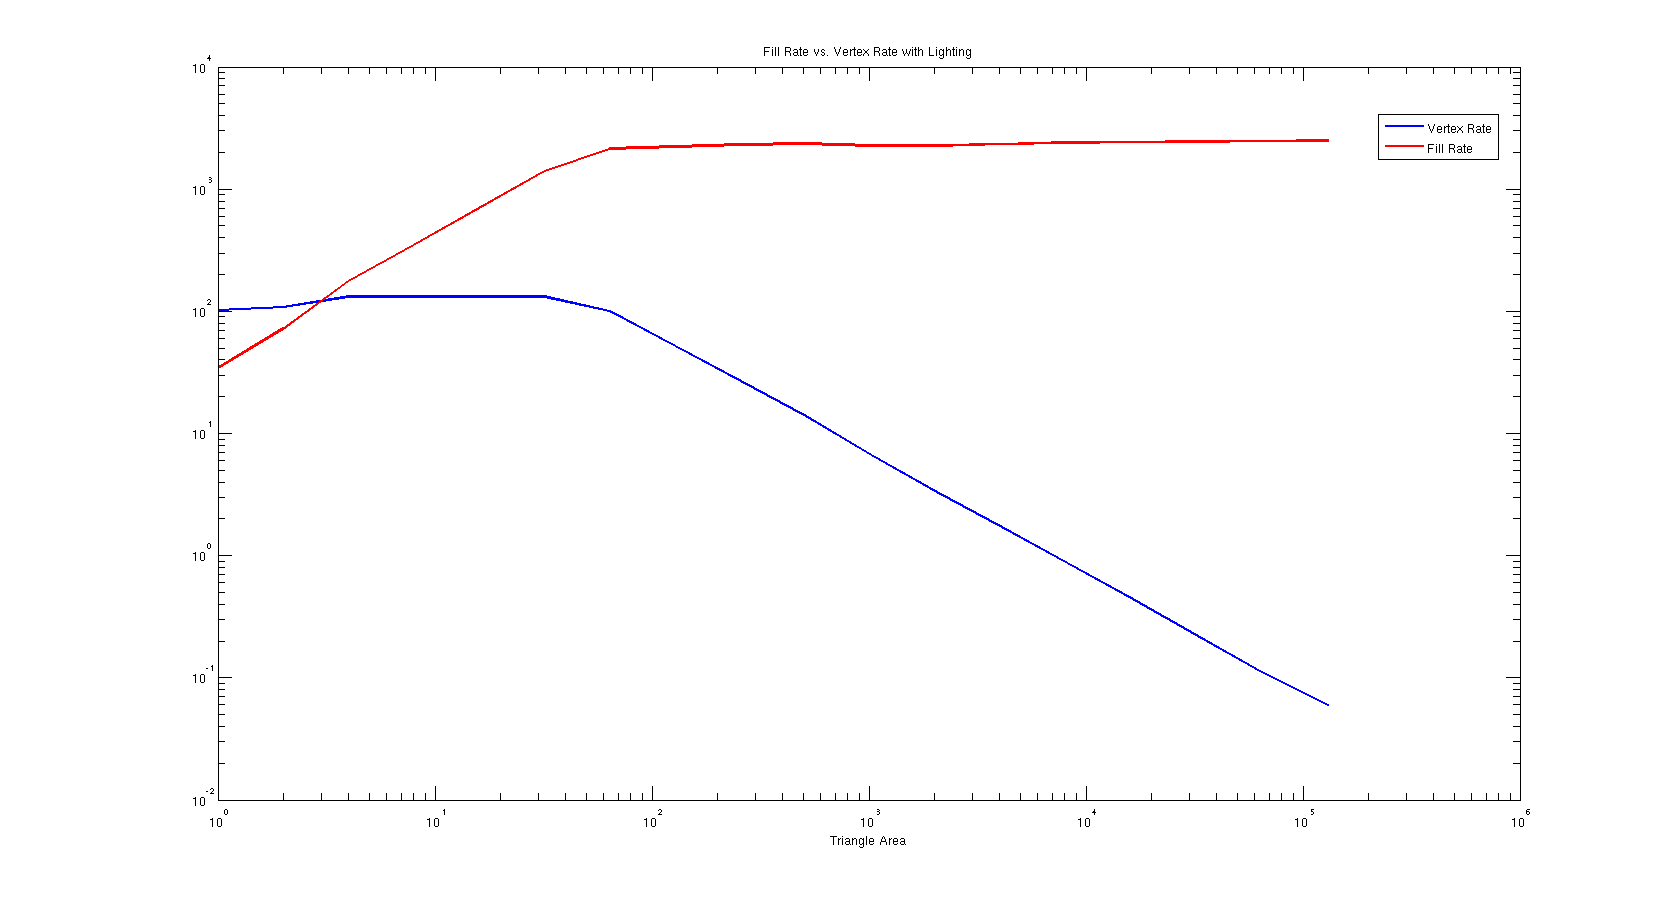
\includegraphics[width=5in]{figures/results2-lighting.png}
	\caption{Vertex and fill rate for various triangle areas with lighting.}
\end{figure}
\FloatBarrier

\begin{figure}[ht!]
	\centering
	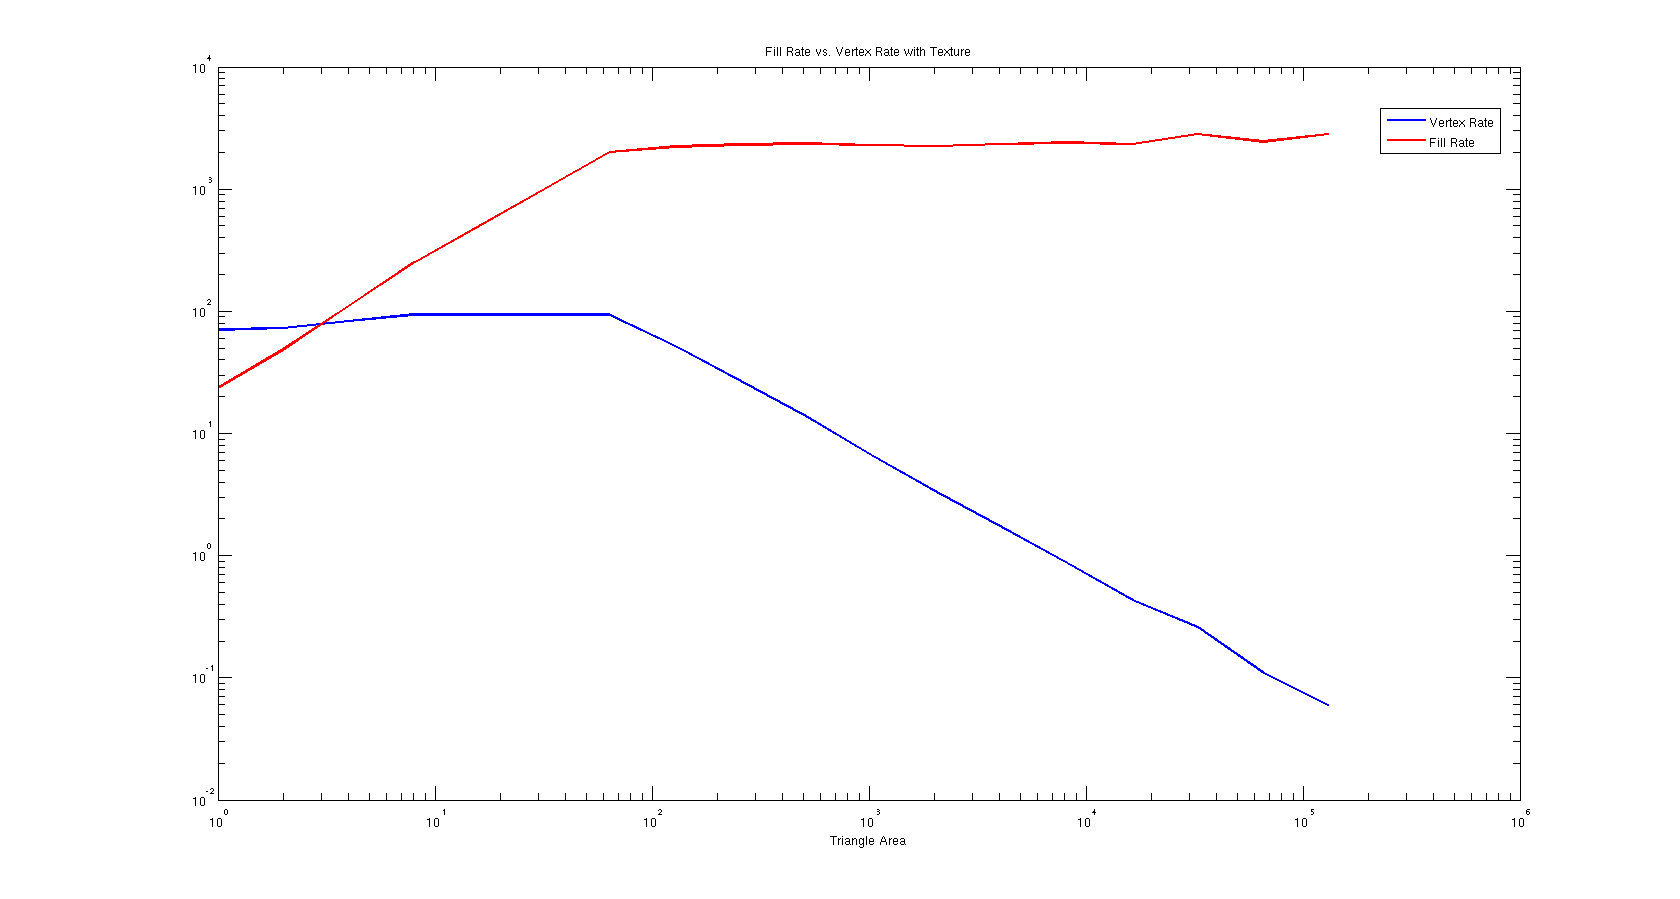
\includegraphics[width=5in]{figures/results2-texture.png}
	\caption{Vertex and fill rate for various triangle areas with texture.}
\end{figure}
\FloatBarrier

\begin{figure}[ht!]
	\centering
	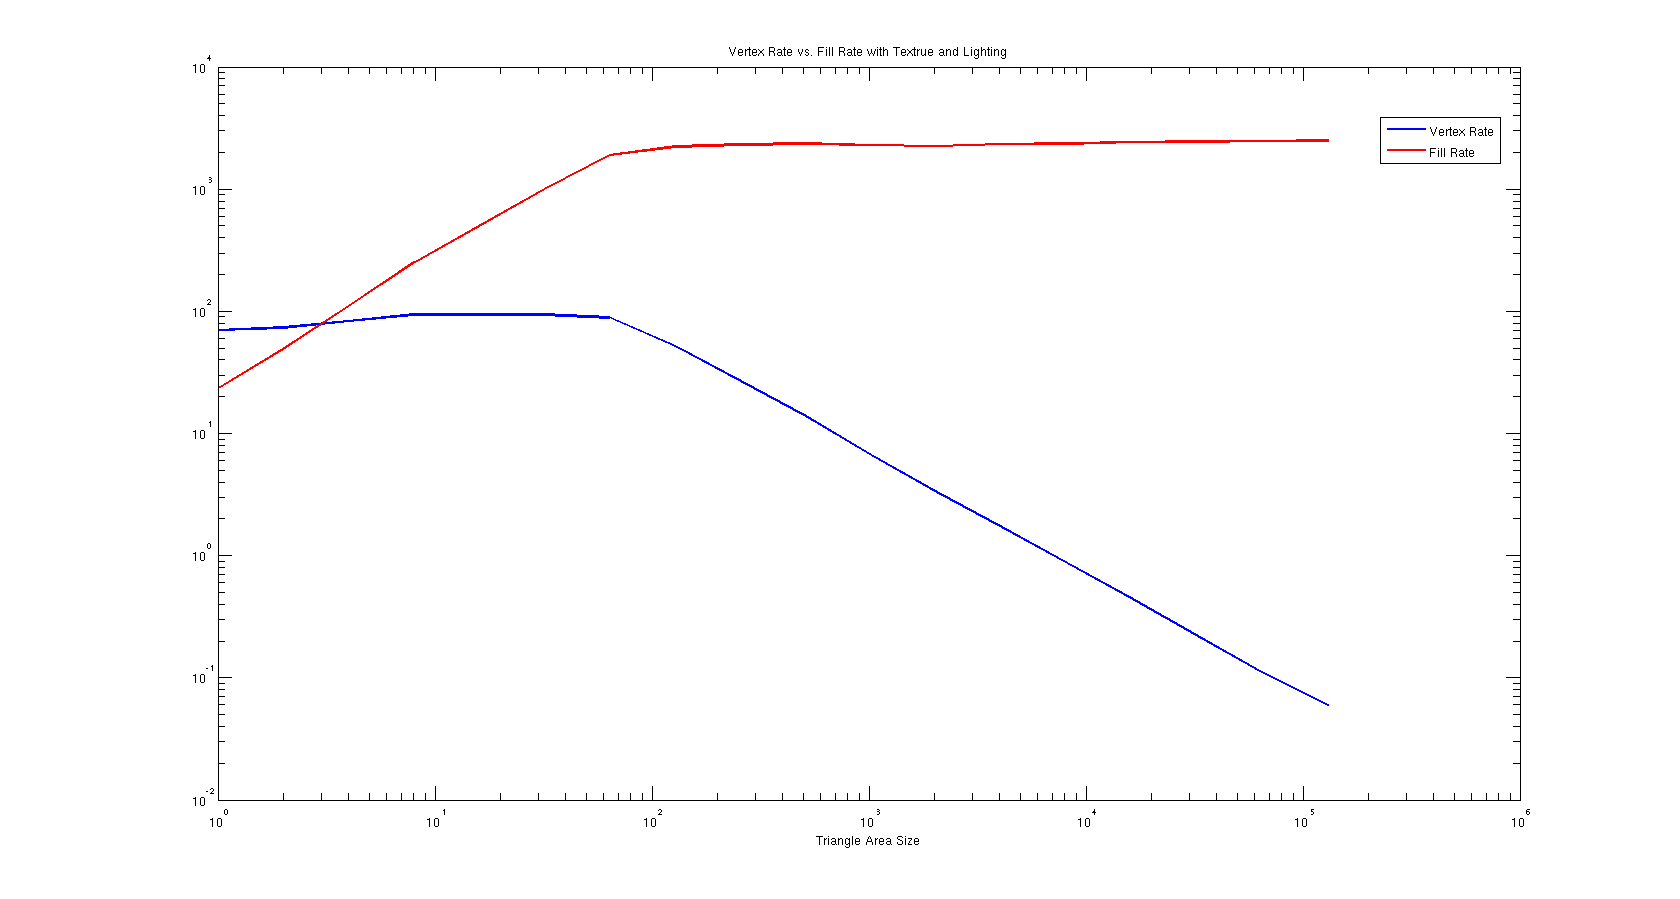
\includegraphics[width=5in]{figures/results2-texture-and-light.png}
	\caption{Vertex and fill rate for various triangle areas with lighting and texture.}
\end{figure}
\FloatBarrier


\subsection{Triangle Types}
This tests the effect of sending triangles to the GPU by using disjoint or triangle strips. Figure 5 shows the vertex rate vs. the fill rate using disjoint triangles and appears exactly the same as all the other graphs, since disjoint triangles are the default for the tests. The vertex rate vs the fill rate for triangle strips are shown in Figure 6. Note that the crossover point shifts down to a triangle area of 16px due to the efficiency of triangle strips.
\begin{figure}[ht!]
	\centering
	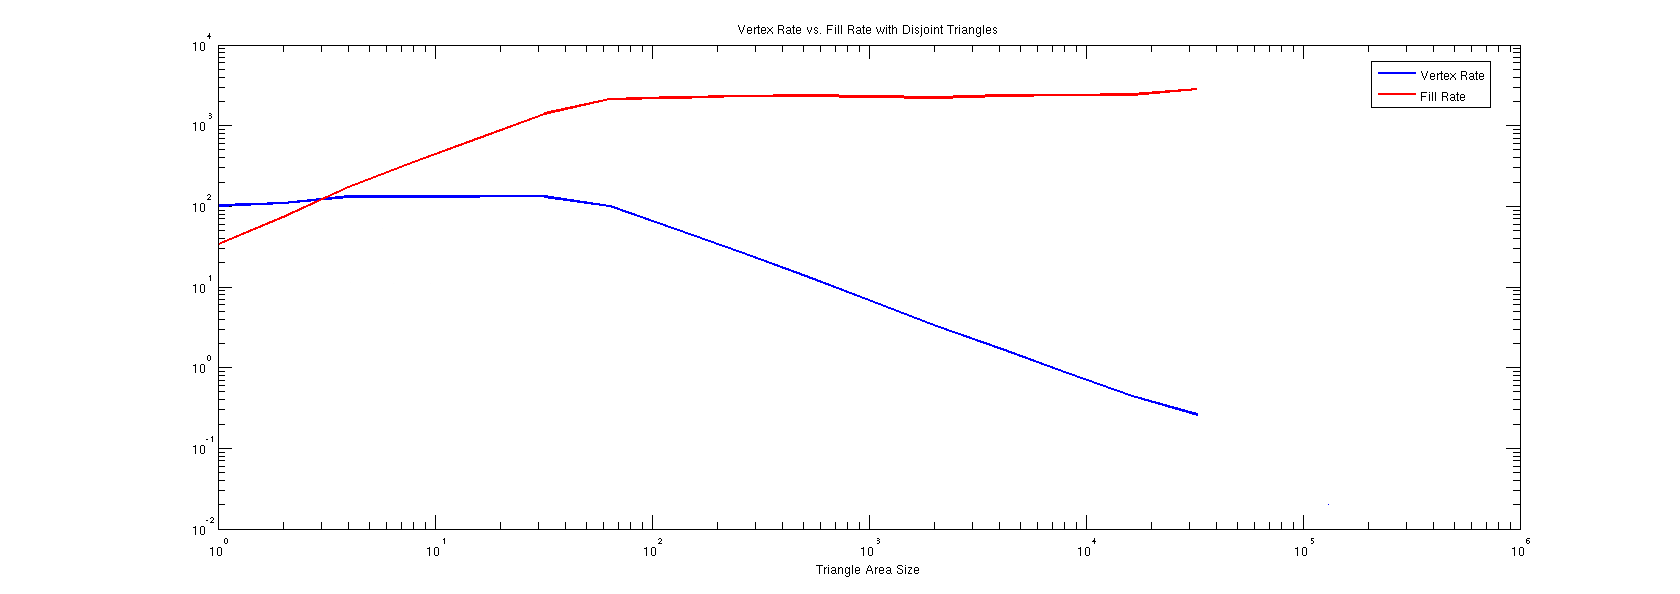
\includegraphics[width=5in]{figures/results2-disjoint-triangles.png}
	\caption{Vertex and fill rate for various triangle areas with disjoint triangles.}
\end{figure}
\FloatBarrier

\begin{figure}[ht!]
	\centering
	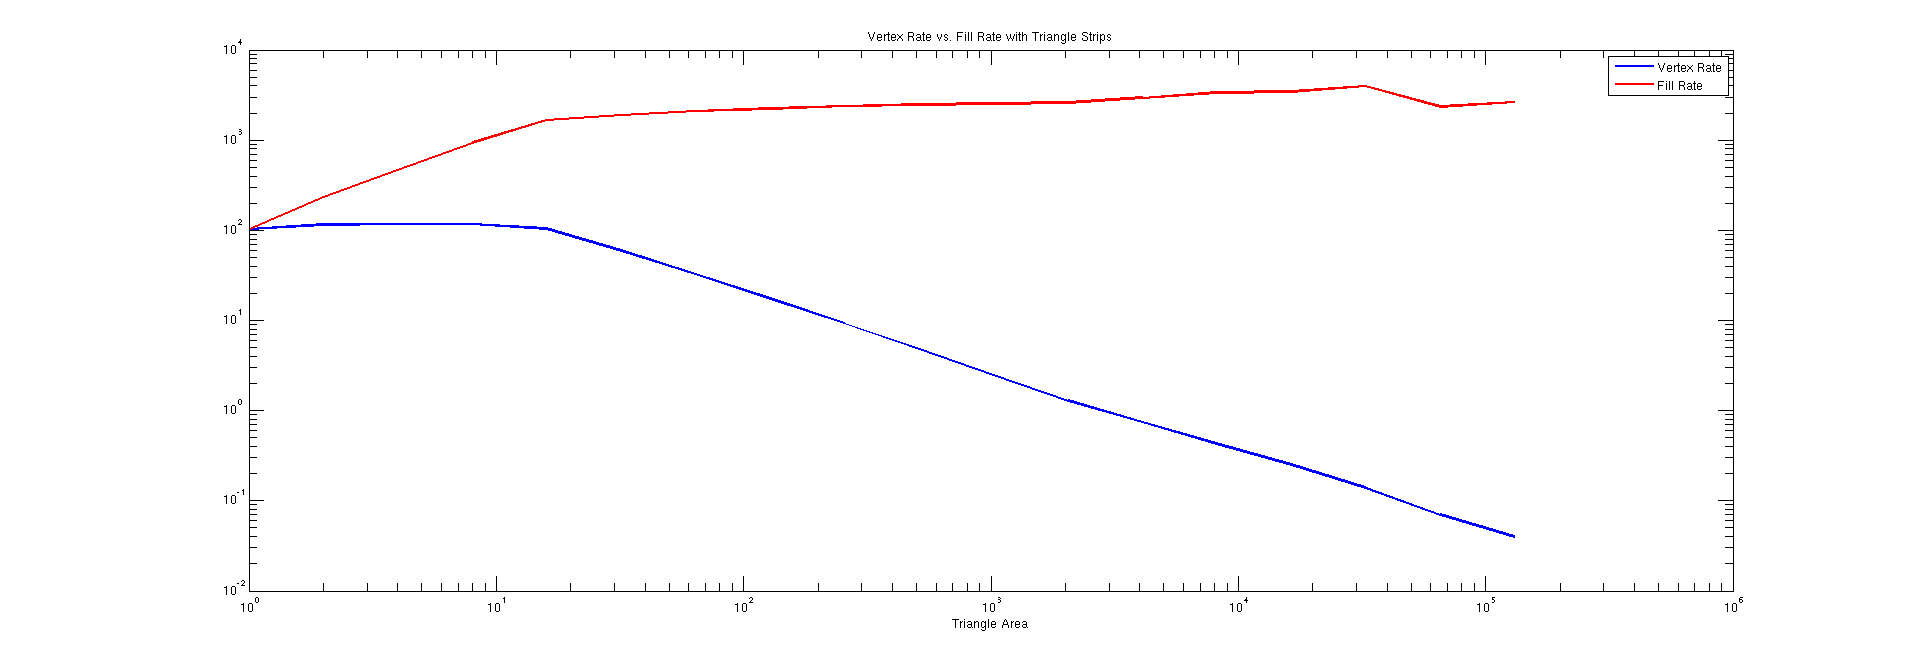
\includegraphics[width=5in]{figures/results2-triangle-strips.png}
	\caption{Vertex and fill rate for various triangle areas with triangle strips.}
\end{figure}
\FloatBarrier

\subsection{Input Bandwidth}
In this test, the program varies the number of vertices per bucket and records the associated vertex rate. The vertex rate increases as the vertices per bucket increases until it flattens around 128 vertices per bucket, as seen in Figure 7. This indicates that, at first, the interface between the CPU and the GPU is the bottleneck and then it transfers to the geometry stage of the GPU. The second jump occurs because the area of the triangles was reduced to prevent memory overflow. However, the trend is still constant which indicates that the GPU geometry stage is still the bottleneck.
\begin{figure}[ht!]
	\centering
	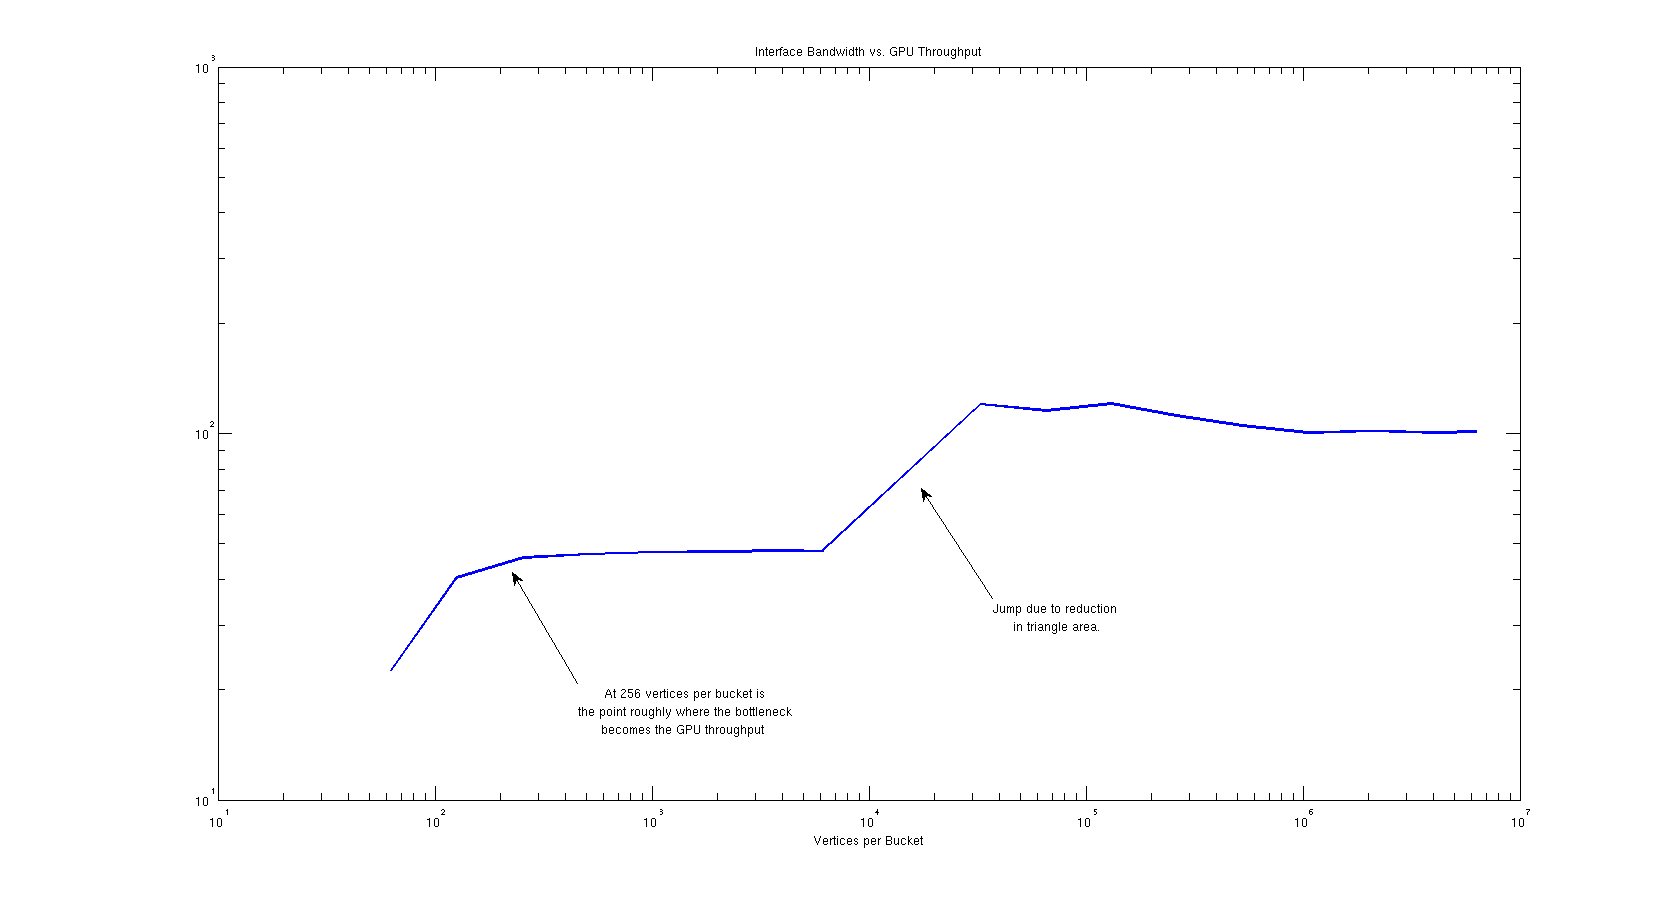
\includegraphics[width=5in]{figures/results3-interface-vs-GPU.png}
	\caption{Vertex rate plotted vs the number of vertices per bucket.}
\end{figure}
\FloatBarrier

\newpage
\subsection{Texture Size}
This test sweeps the size of the texture used and shows how the fill rate changes, as seen in Figure 8. In particular, the fill rate suffers as the texture size increases. The tipping point is when the texture size reaches about 256 px. At that point, the fill rate begins to reduce more rapidly as the texture lookups hinder the rasterizer.
\begin{figure}[ht!]
	\centering
	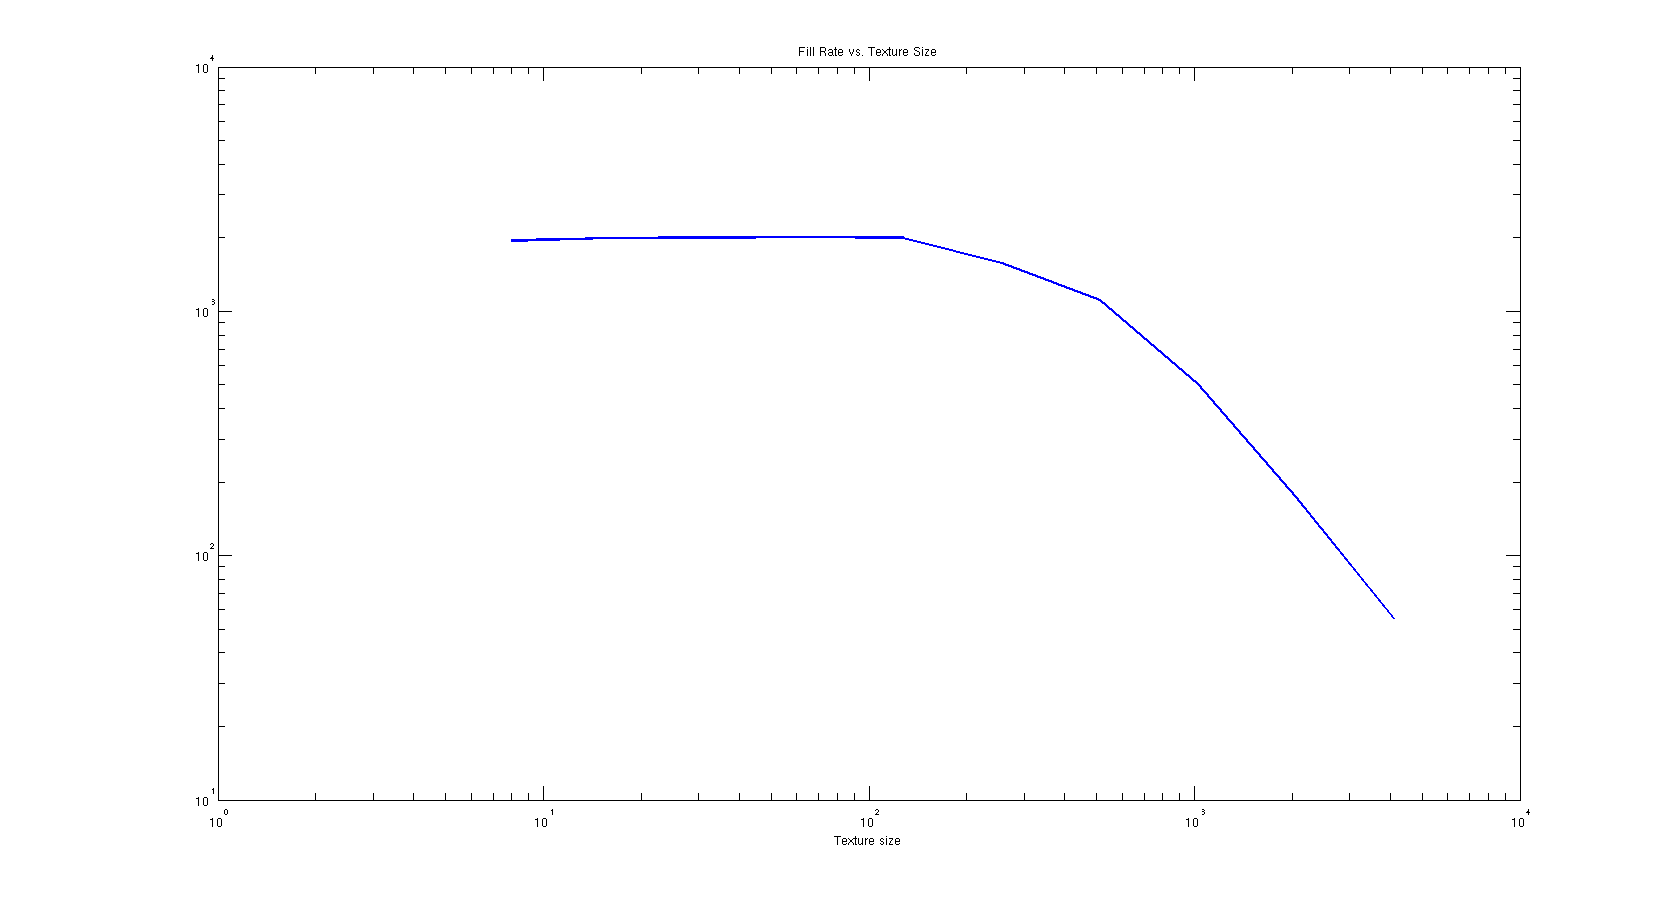
\includegraphics[width=5in]{figures/results4-fill-rate-vs-texture.png}
	\caption{Fill rate for texture sizes.}
\end{figure}
\FloatBarrier

% Part B ----------------------------------------------------------------------
\clearpage
\newpage
\section{Part B}
In Part B, we examine the general purpose graphics processing unit(GPGPU) capabilities of the graphics card with a particular focus on the compute performance as characterized by the floating point operations per second (FLOPS), often represented in GigaFLOPS (GFLOPS). This part of the assignment primarily used CUDA to generate GPGPU code.


\subsection{Maximum FLOPS}
The maximum number of FLOPS capable by the graphics card is 87 GFLOPS. This data was found by creating a kernel to operate on the GPU that performed many register arithmetic operations and wrote those to a location in memory at the end.


\subsection{Memory Bandwidth}
The maximum memory bandwidth of the graphics card is 9.4 GB/s. We tested this by creating a kernel which copies an input array into an output array in a coalescing-friendly way amongst threads.

\newpage
\subsection{Effect of Blocks on FLOPS}
This test examined how the number of blocks used affected the maximum FLOPS. To perform this test, the same kernel as the maximum FLOPS test was used but the number of blocks were altered for each complete run to obtain a full data set. As the number of blocks increases, the maximum FLOPS oscillate but increase, as seen in Figure 9. The oscillations occur as the number of block get closer or further from maximum occupancy. The overall increase occurs because more blocks mean more threads and more threads correspond to a higher minimum utilization. From this data, we can conclude that the GPU we are using has 4 multiprocessors since the maximum performance per blocks occurs when the number of blocks reaches 4.


\begin{figure}[ht!]
	\centering
	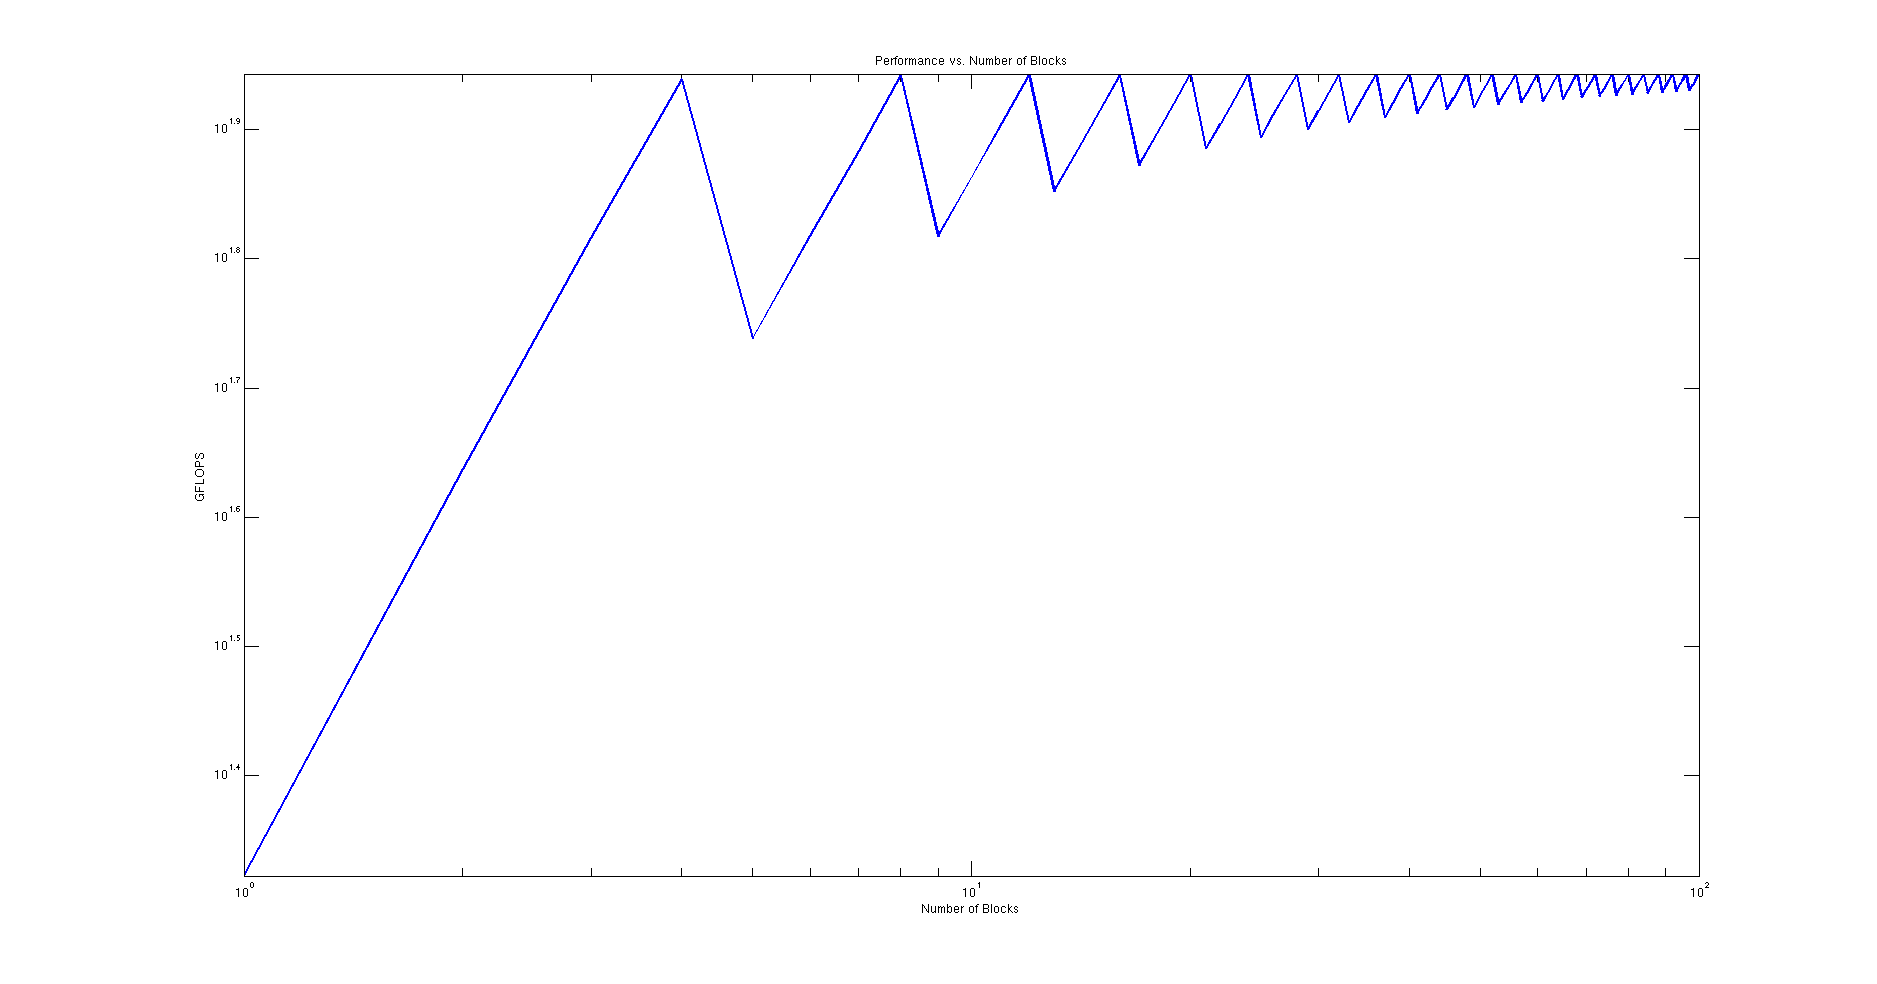
\includegraphics[width=5in]{figures/blocks_v_perf.png}
	\caption{Performance (GFLOPS) vs. Number of Blocks.}
\end{figure}
\FloatBarrier

\newpage
\subsection{Effect of Warps on FLOPS}
This test altered the number of warps (groups of 32 threads) and recorded the maximum FLOPS at each of these points. The number of warps affected the FLOPS by increasing the number of threads which allows more data to run on the multiprocessors (until it reaches the GPU max FLOPS ceiling), as shown in Figure 10. The small oscillations occur because the warps cannot be mapped in a way that causes full occupancy for all possible values.

\begin{figure}[ht!]
	\centering
	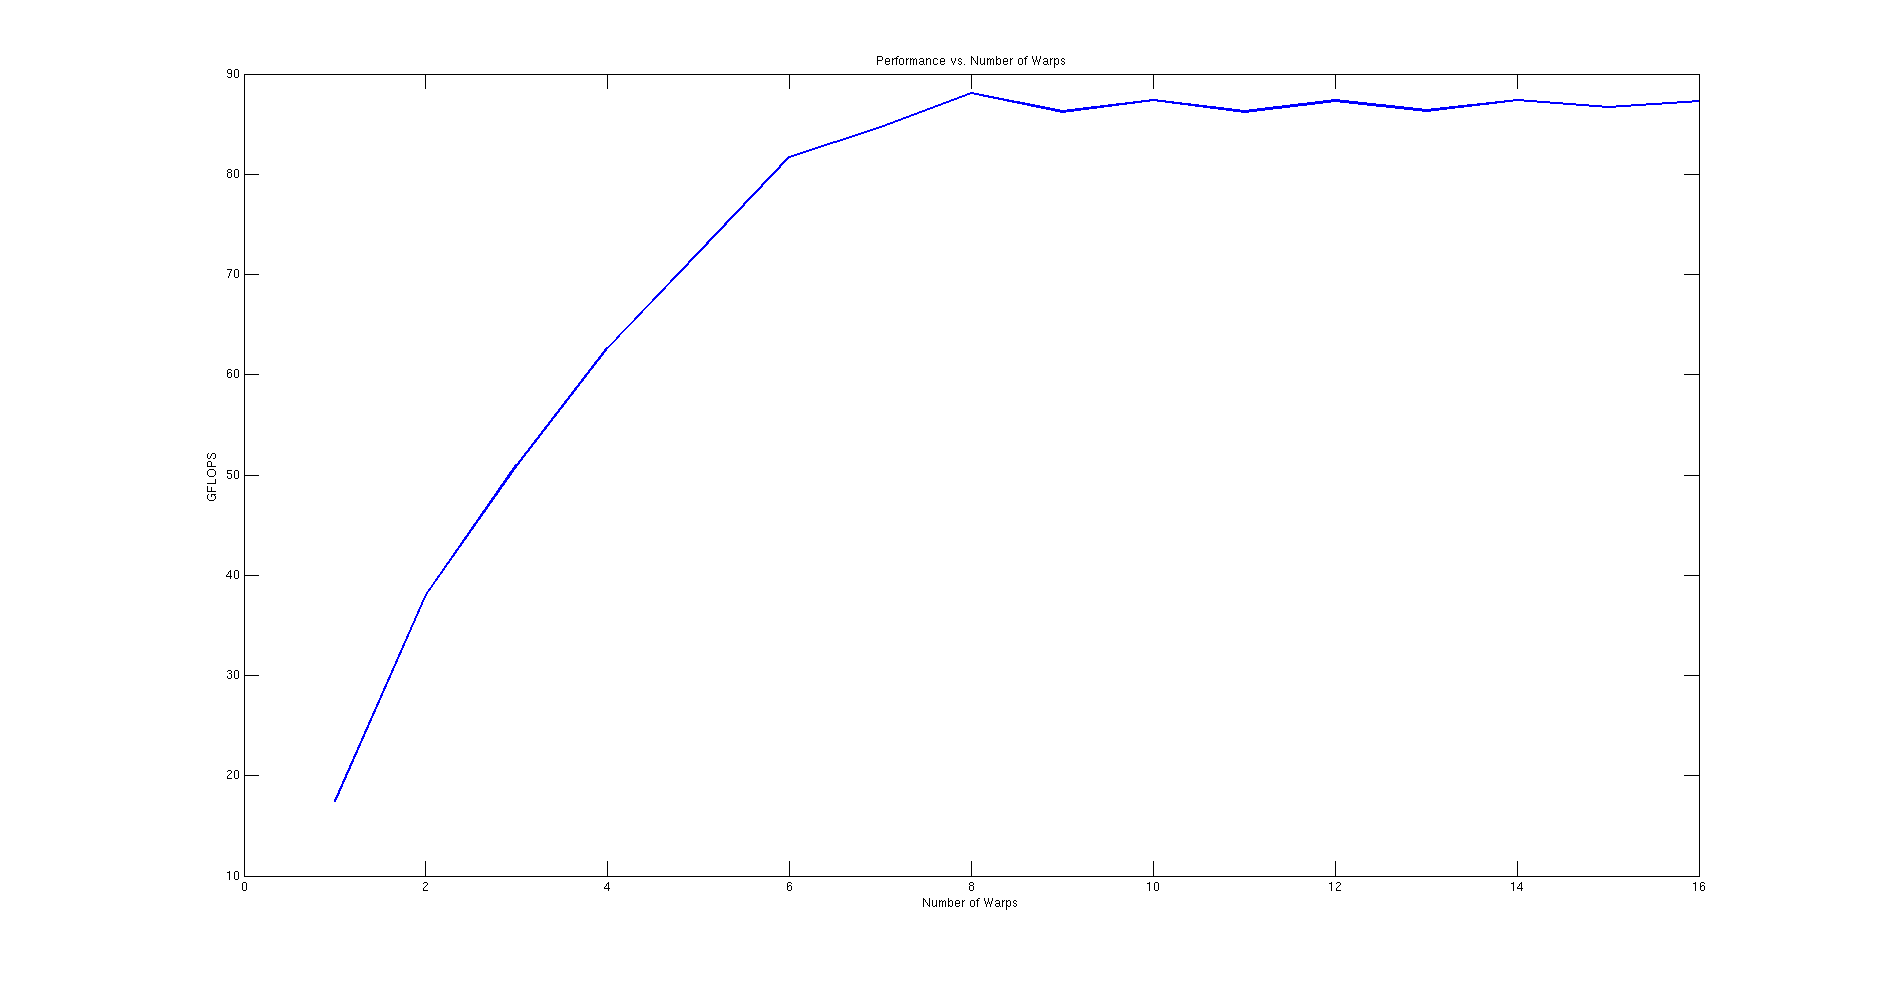
\includegraphics[width=5in]{figures/warps_v_perf.png}
	\caption{Performance (GFLOPS) vs. Number of Warps}
\end{figure}
\FloatBarrier

\subsection{Effect of Branch Granularity on FLOPS}
This test changed the branch granularity within a defined kernel (that supported up to 32 branches) and measured the number of FLOPS that resulted from it. The specialized kernel used part of the FLOPS test from before but added a part that would be changed based on which branch was taken. As seen in Figure 11, the higher the branch granularity is, the worse the FLOPS become. This occurs because a higher branch granularity requires the other threads in the warp to stall while the branching threads complete their execution. This applies for each potential branch path that the threads in a warp take so more paths (called granularity) results in more stalling while the different paths are computed. The curve of the data in Figure 11 occurs because as more branch directions are added, the overall effect of each direction on the average thread execution time is marginally reduced.

\begin{figure}[ht!]
	\centering
	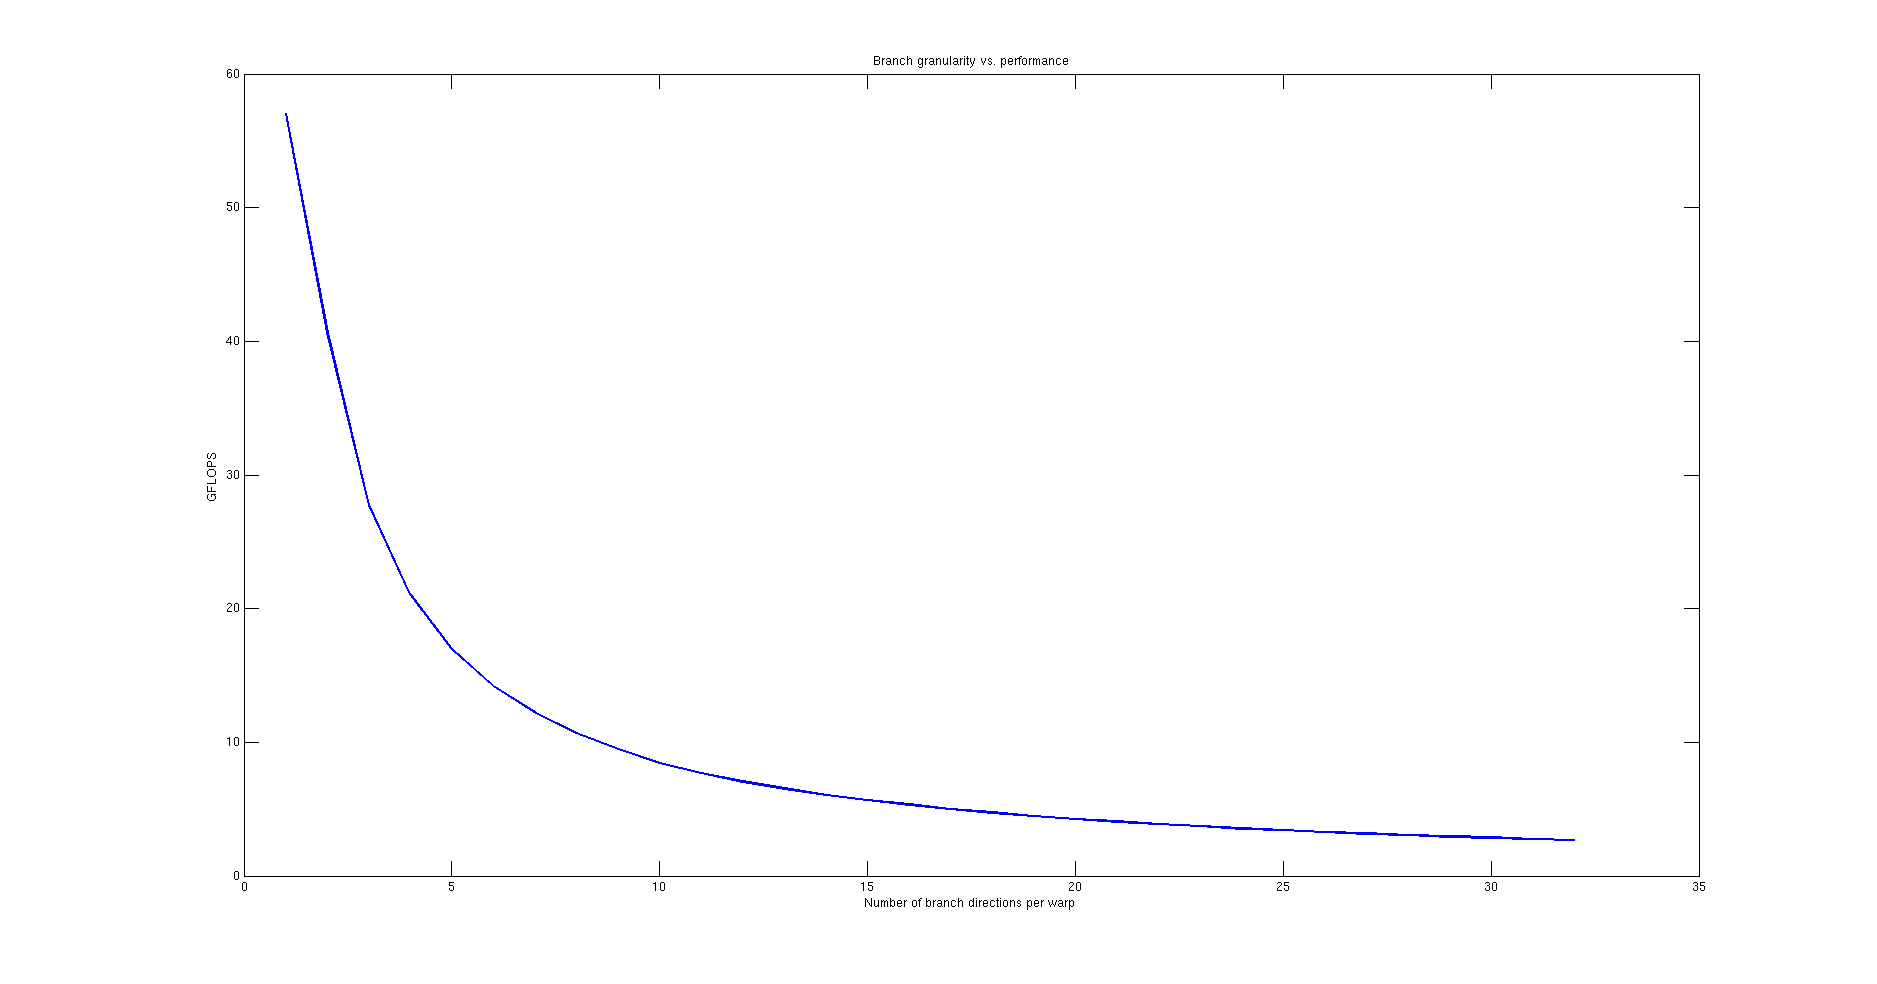
\includegraphics[width=5in]{figures/branch_v_perf.png}
	\caption{Performance (GFLOPS) vs. Branch Granularity.}
\end{figure}
\FloatBarrier

\subsection{Effect of Persistent Threads on FLOPS}
The final test compared the use of persistent threads, using threads that matched to the hardware rather than to the work needed to be done, with the standard CUDA approach, which maps one thread to one piece of work that needs to be completed. As a result of this test, we saw a speedup using persistent threads from 87 GFLOPS to 89 GFLOPS, a 2.3\% speedup.

% References -----------------------------------------------------------------
\clearpage
\section{Code}
\begin{center}
	The code can be found on our GitHub repository:

	\url {https://github.com/phil-monroe/EEC-277---Project-2}
\end{center}

The code is organized into multiple folders. The code for parts A and B can be found in the part\_a and part\_b folders respectively. The CUDA codes for part b are also arranged in a series of folders based on what that code is testing.

\end{document}